\documentclass{abntex2}

% essa linha eh um comentario!

\usepackage[brazil]{babel}  % traducao da formatacao
\usepackage[utf8]{inputenc}  % acentuacao

\usepackage{graphicx}  % figuras
\usepackage{subcaption}  % subfigure

\usepackage{lipsum}  % gerador de lero-lero

\usepackage[alf]{abntex2cite} % Citações padrão ABNT

\usepackage{amsthm}  % coisas matematicas
\newtheorem{definicao}{Definição}[section]  % ambiente definicao
\newtheorem{teorema}{Teorema}[chapter]  % ambiente teorema

% informacoes da capa
\autor{Adriano}
\titulo{Meu querido TCC}
\data{21 agosto de 2018}
\instituicao{UFGD}

\makeindex

\begin{document}
\imprimircapa  % capa

\imprimirfolhaderosto*  % folha de rosto

% ficha catalografica
\begin{fichacatalografica}
	\sffamily
	\vspace*{\fill}					% Posição vertical
	\begin{center}					% Minipage Centralizado
	\fbox{\begin{minipage}[c][8cm]{13.5cm}		% Largura
	\small
	\imprimirautor
	%Sobrenome, Nome do autor
	
	\hspace{0.5cm} \imprimirtitulo  / \imprimirautor. --
	\imprimirlocal, \imprimirdata-
	
	\hspace{0.5cm} \thelastpage p. : il. (algumas color.) ; 30 cm.\\
	
	\hspace{0.5cm} \imprimirorientadorRotulo~\imprimirorientador\\
	
	\hspace{0.5cm}
	\parbox[t]{\textwidth}{\imprimirtipotrabalho~--~\imprimirinstituicao,
	\imprimirdata.}\\
	
	\hspace{0.5cm}
		1. Palavra-chave1.
		2. Palavra-chave2.
		2. Palavra-chave3.
		I. Orientador.
		II. Universidade xxx.
		III. Faculdade de xxx.
		IV. Título 			
	\end{minipage}}
	\end{center}
\end{fichacatalografica}

% folha de aprovacao
\begin{folhadeaprovacao}

  \begin{center}
    {\ABNTEXchapterfont\large\imprimirautor}

    \vspace*{\fill}\vspace*{\fill}
    \begin{center}
      \ABNTEXchapterfont\bfseries\Large\imprimirtitulo
    \end{center}
    \vspace*{\fill}
    
    \hspace{.45\textwidth}
    \begin{minipage}{.5\textwidth}
        \imprimirpreambulo
    \end{minipage}%
    \vspace*{\fill}
   \end{center}
        
   Trabalho aprovado. \imprimirlocal, 24 de novembro de 2012:

   \assinatura{\textbf{\imprimirorientador} \\ Orientador} 
   \assinatura{\textbf{Professor} \\ Convidado 1}
   \assinatura{\textbf{Professor} \\ Convidado 2}
   %\assinatura{\textbf{Professor} \\ Convidado 3}
   %\assinatura{\textbf{Professor} \\ Convidado 4}
      
   \begin{center}
    \vspace*{0.5cm}
    {\large\imprimirlocal}
    \par
    {\large\imprimirdata}
    \vspace*{1cm}
  \end{center}
  
\end{folhadeaprovacao}

% dedicatoria
\begin{dedicatoria}
   \vspace*{\fill}
   \centering
   \noindent
   \textit{ Este trabalho é dedicado às crianças adultas que,\\
   quando pequenas, sonharam em se tornar cientistas.} \vspace*{\fill}
\end{dedicatoria}

% agradecimentos
\begin{agradecimentos}
\lipsum[1]
\end{agradecimentos}

% resumo
\setlength{\absparsep}{18pt} % ajusta o espaçamento dos parágrafos do resumo
\begin{resumo}
\lipsum[2]

 \textbf{Palavras-chave}: latex. abntex. editoração de texto.
\end{resumo}

% resumo em inglês
\begin{resumo}[Abstract]
	\begin{otherlanguage*}{english}
		\lipsum[2]

		\textbf{Keywords}: latex. abntex. text editoration.
	\end{otherlanguage*}
\end{resumo}

% lista de figuras
\pdfbookmark[0]{\listfigurename}{lof}
\listoffigures*
\cleardoublepage

% lista de tabelas
\pdfbookmark[0]{\listtablename}{lot}
\listoftables*
\cleardoublepage

% lista de abreviaturas e siglas
\begin{siglas}
  \item[ABNT] Associação Brasileira de Normas Técnicas
  \item[abnTeX] ABsurdas Normas para TeX
\end{siglas}

% lista de símbolos
\begin{simbolos}
  \item[$ \Gamma $] Letra grega Gama
  \item[$ \Lambda $] Lambda
  \item[$ \zeta $] Letra grega minúscula zeta
  \item[$ \in $] Pertence
\end{simbolos}

% sumario
\pdfbookmark[0]{\contentsname}{toc}
\tableofcontents*
\cleardoublepage

% elementos textuais
\textual

\chapter{Introdução}
\lipsum[1-8]  % lero-lero

\chapter{Matemática: diversão!}
% equacao na mesma linha do texto
Pitágoras: $a^2=b^2+c^2$

% equacao centralizada
$$a^2=b^2+c^2$$

% equacao numerada
\begin{equation}
	a^2=b^2+c^2
	\label{pitagoras}
\end{equation}

\section{Definições e Teoremas}
\begin{definicao}
	Uma \index{antiderivada} de uma função $f$ em $I$ é uma função $F$ tal que $F'(x)=f(x),\forall x\in I$.
\end{definicao}

\begin{teorema}(Teorema Fundamental do Cálculo)
	\[\int_a^b f(x) dx = F(b)-F(a).\]
	\label{tfc}
\end{teorema}
\begin{proof}
	\lipsum[1]
\end{proof}

Pelo Teorema \ref{tfc} e por Pitágoras (equação \ref{pitagoras}), segue o resultado... 

\begin{teorema}
	Esse é mais um teorema...
\end{teorema}

\index{Integral}

\chapter{Figuras}
Vamos inserir figuras:
\begin{figure}[h]
	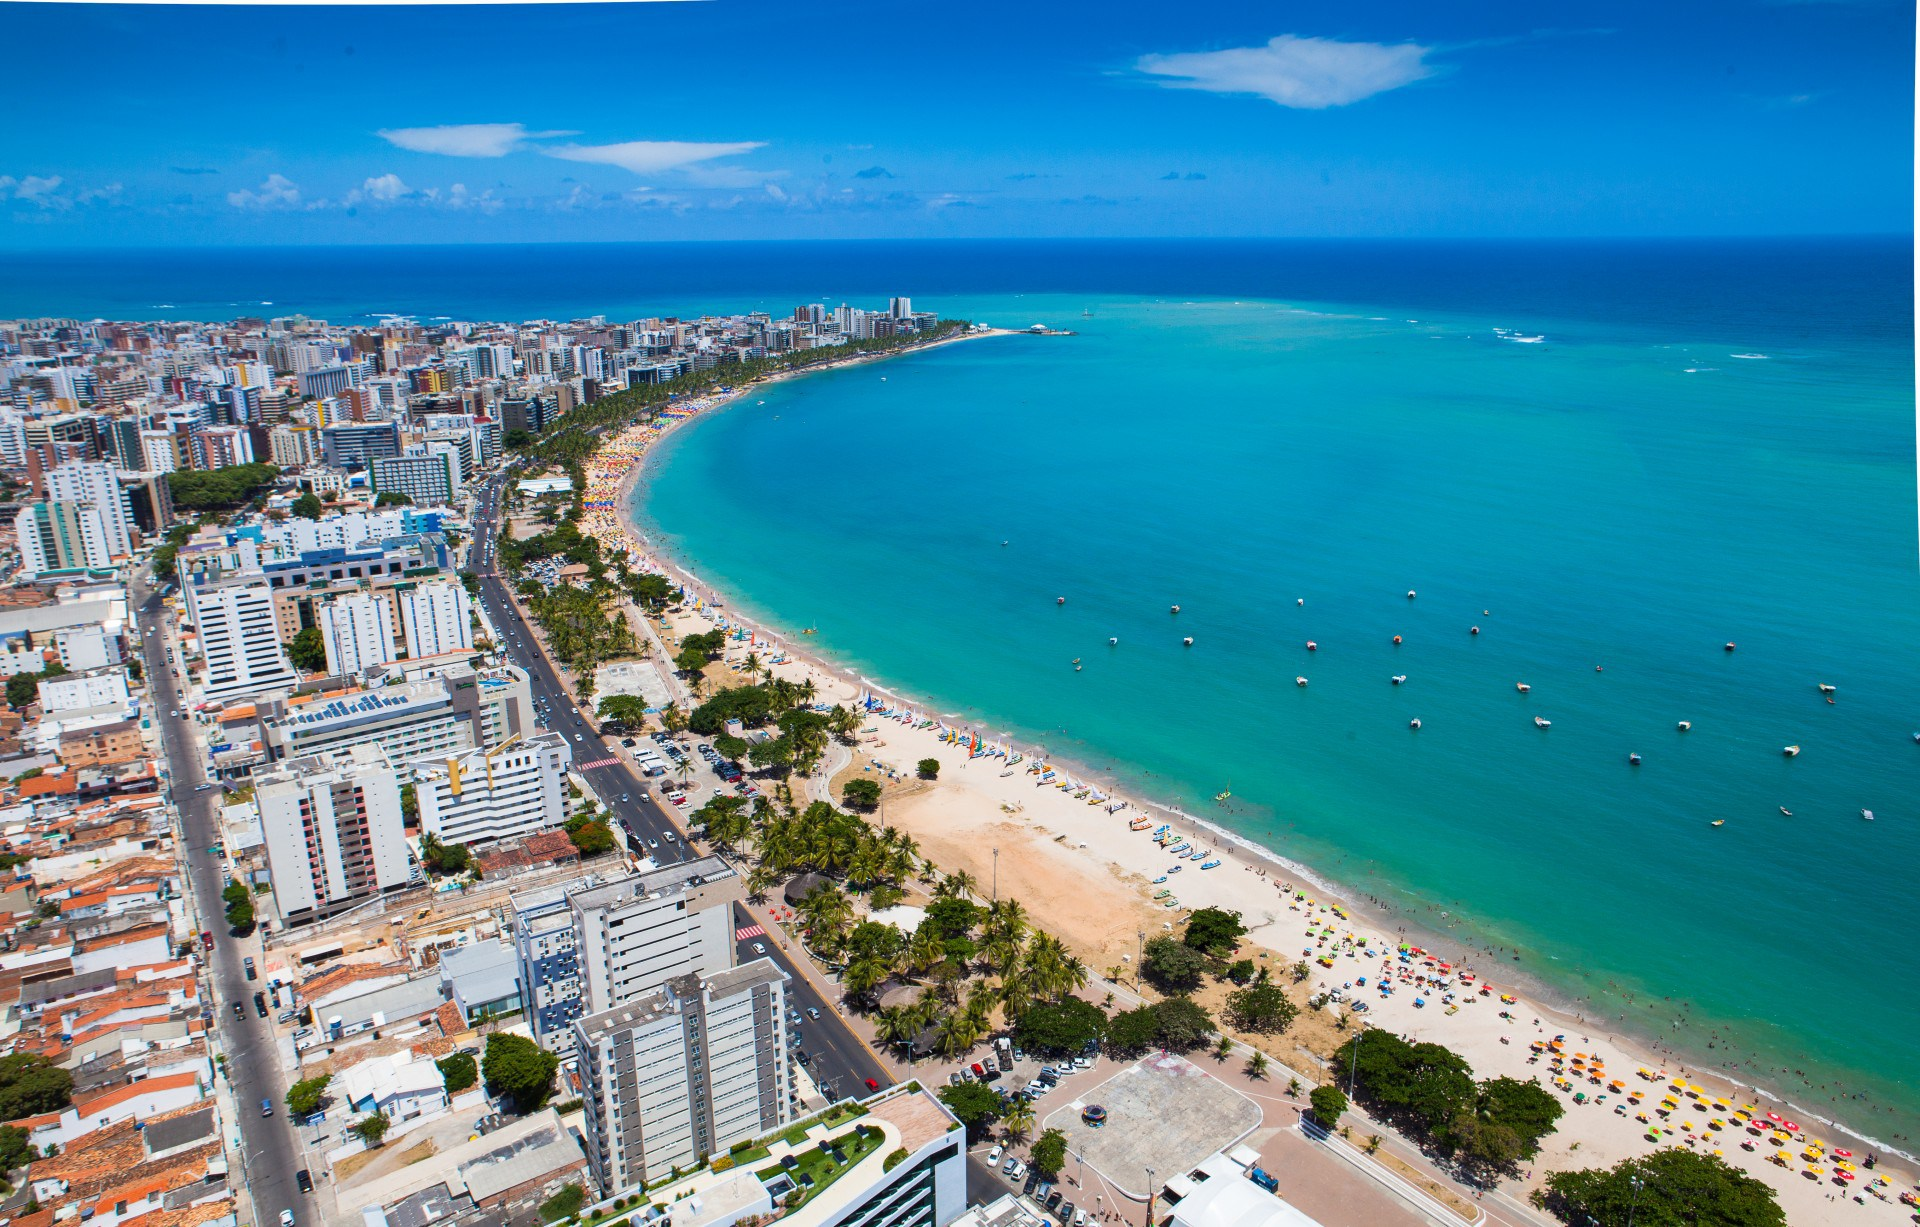
\includegraphics[scale=0.1]{maceio.jpg}
\end{figure}

\begin{figure}[h]
	\centering
	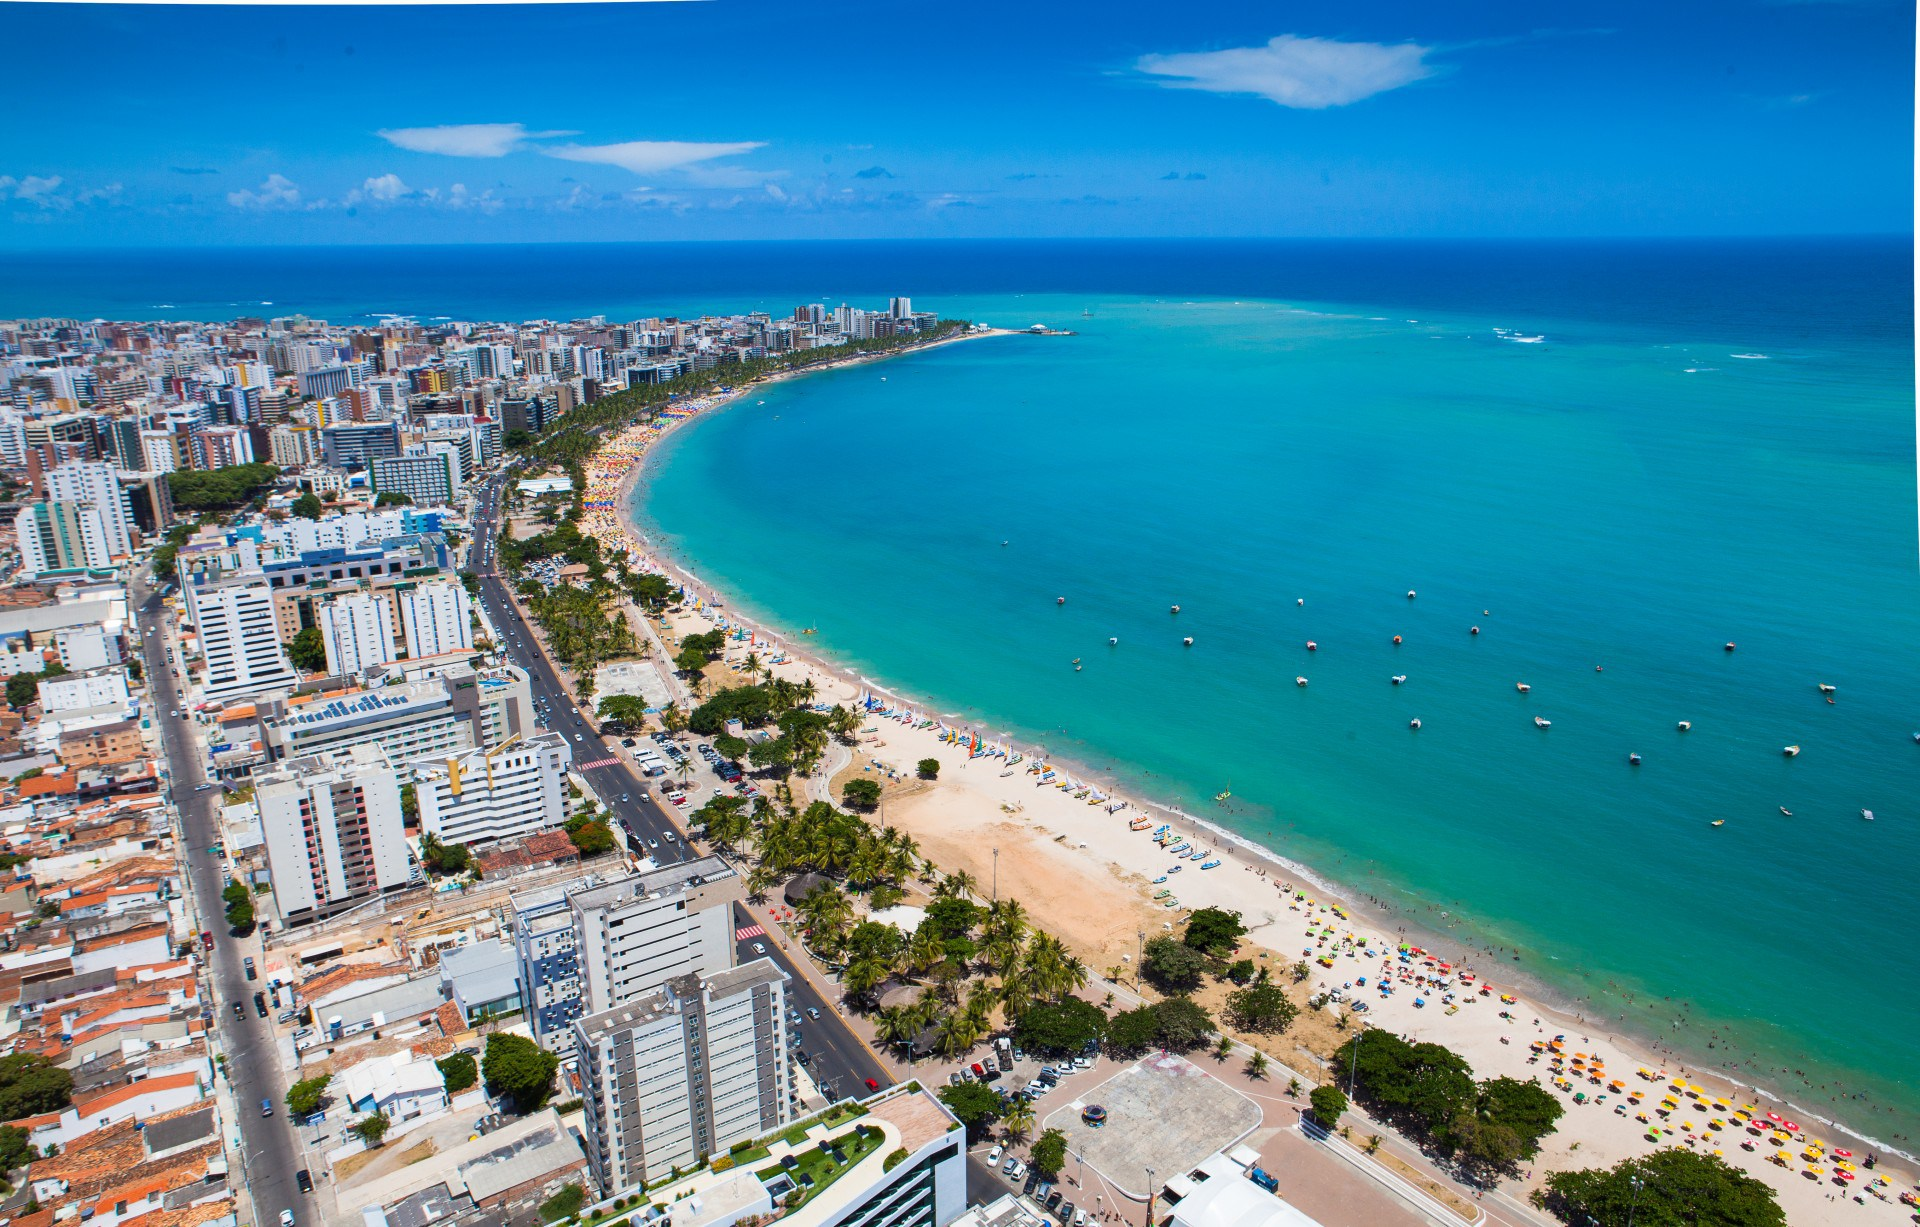
\includegraphics[scale=0.1]{maceio.jpg}
\end{figure}

\begin{figure}[h]
	\flushright
	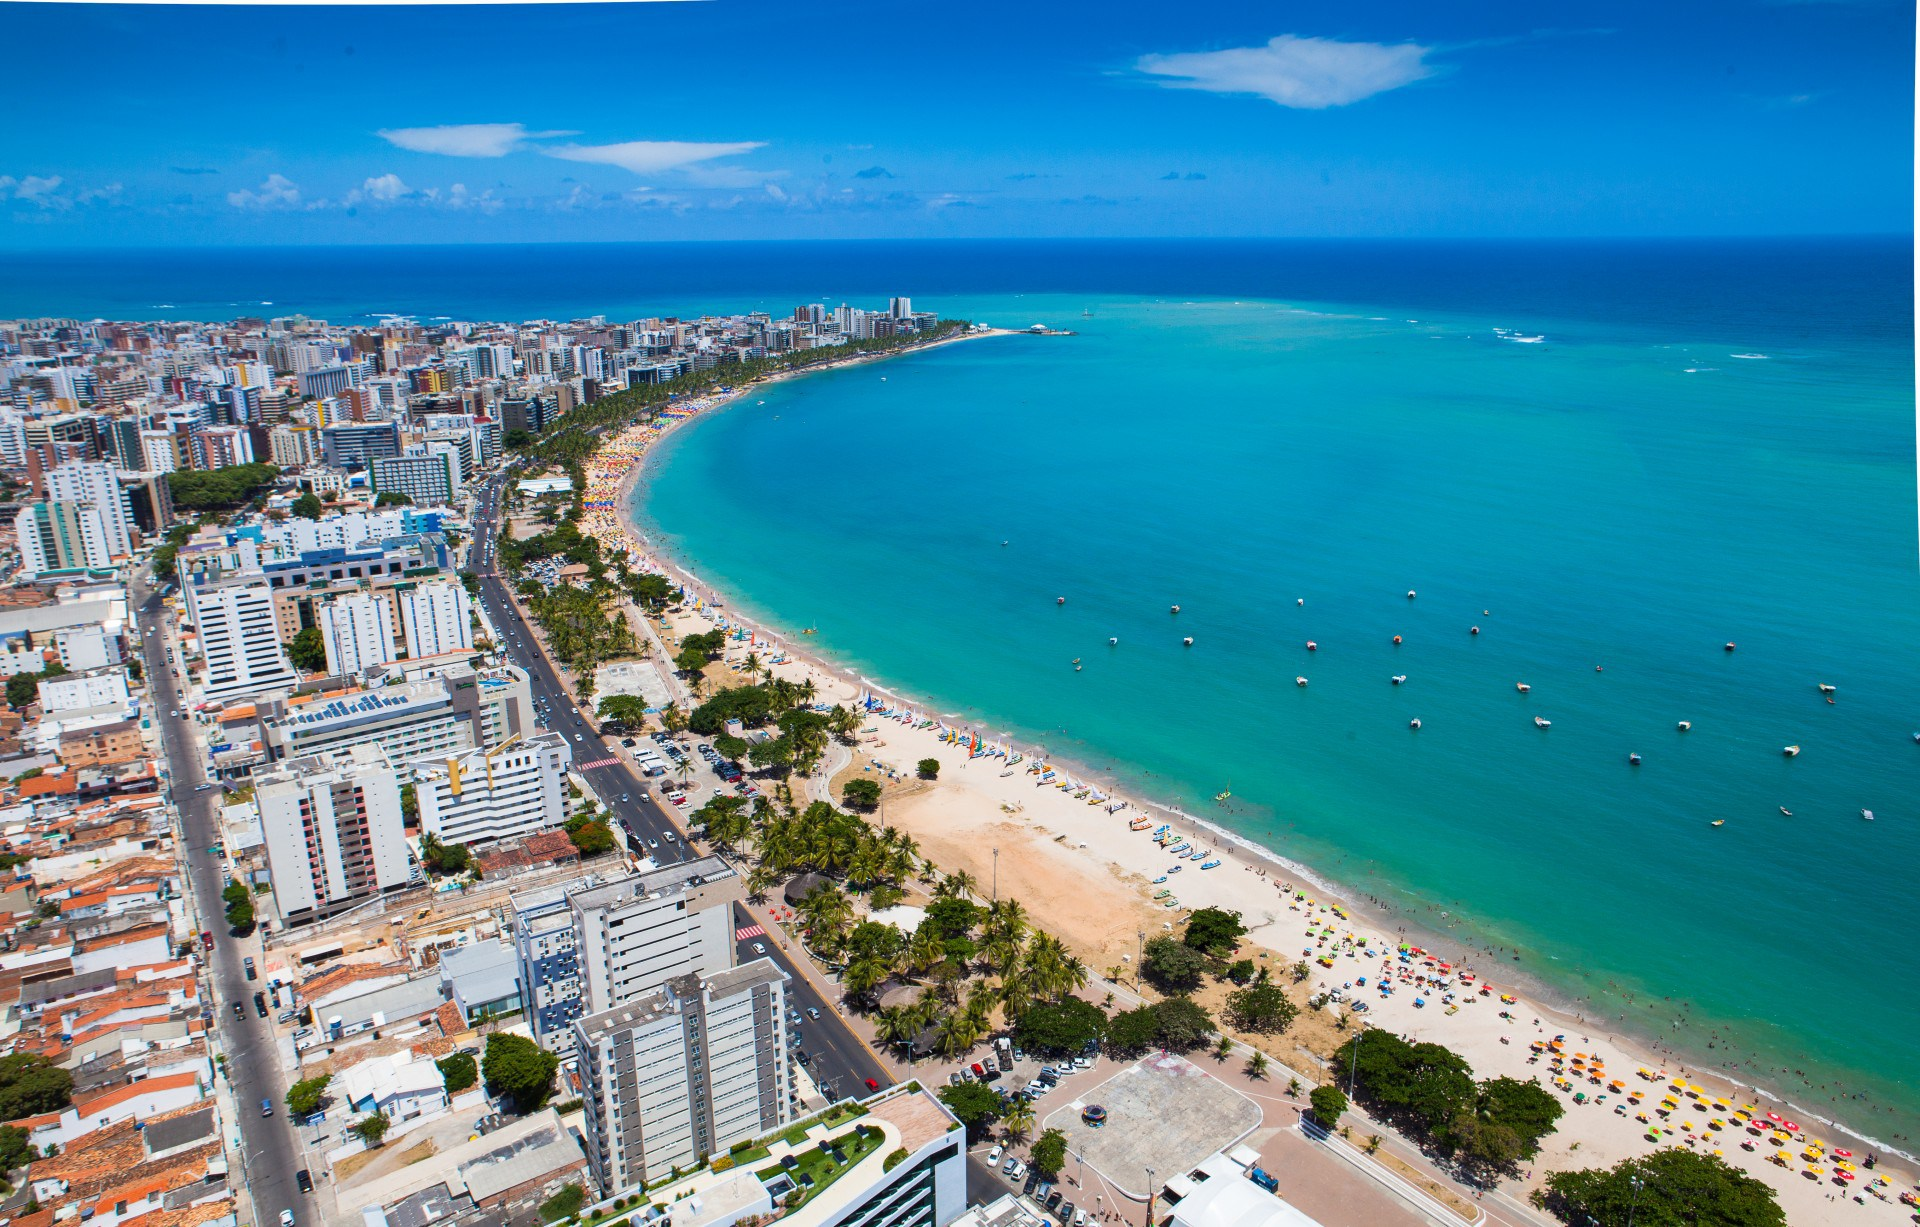
\includegraphics[scale=0.1]{maceio.jpg}
\end{figure}

\begin{figure}[h]
	\centering
	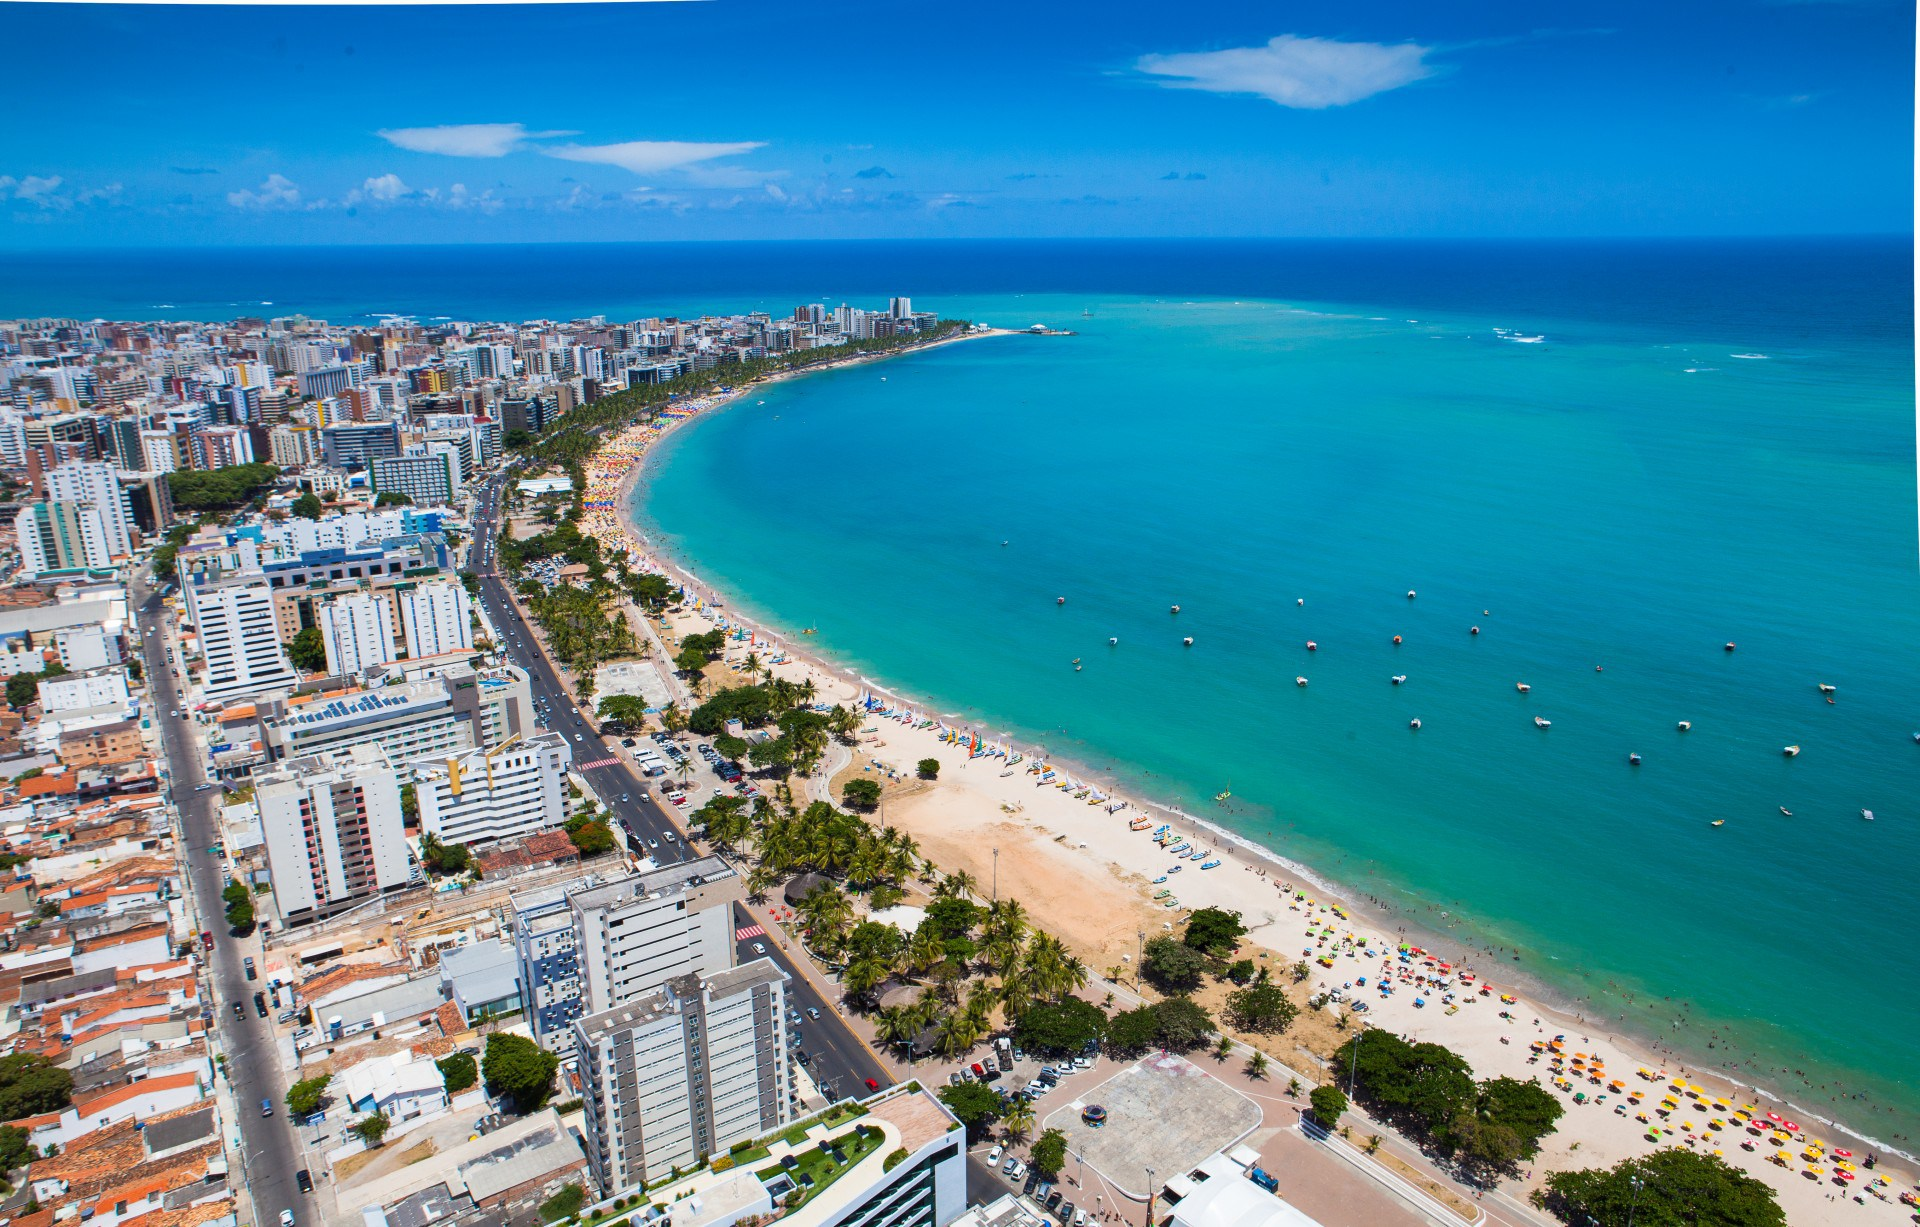
\includegraphics[scale=0.1]{maceio.jpg}
	\caption{Essa figura tem uma legenda.}
\end{figure}

\begin{figure}[h]
	\centering
	\caption{Essa legenda está em cima da figura.}
	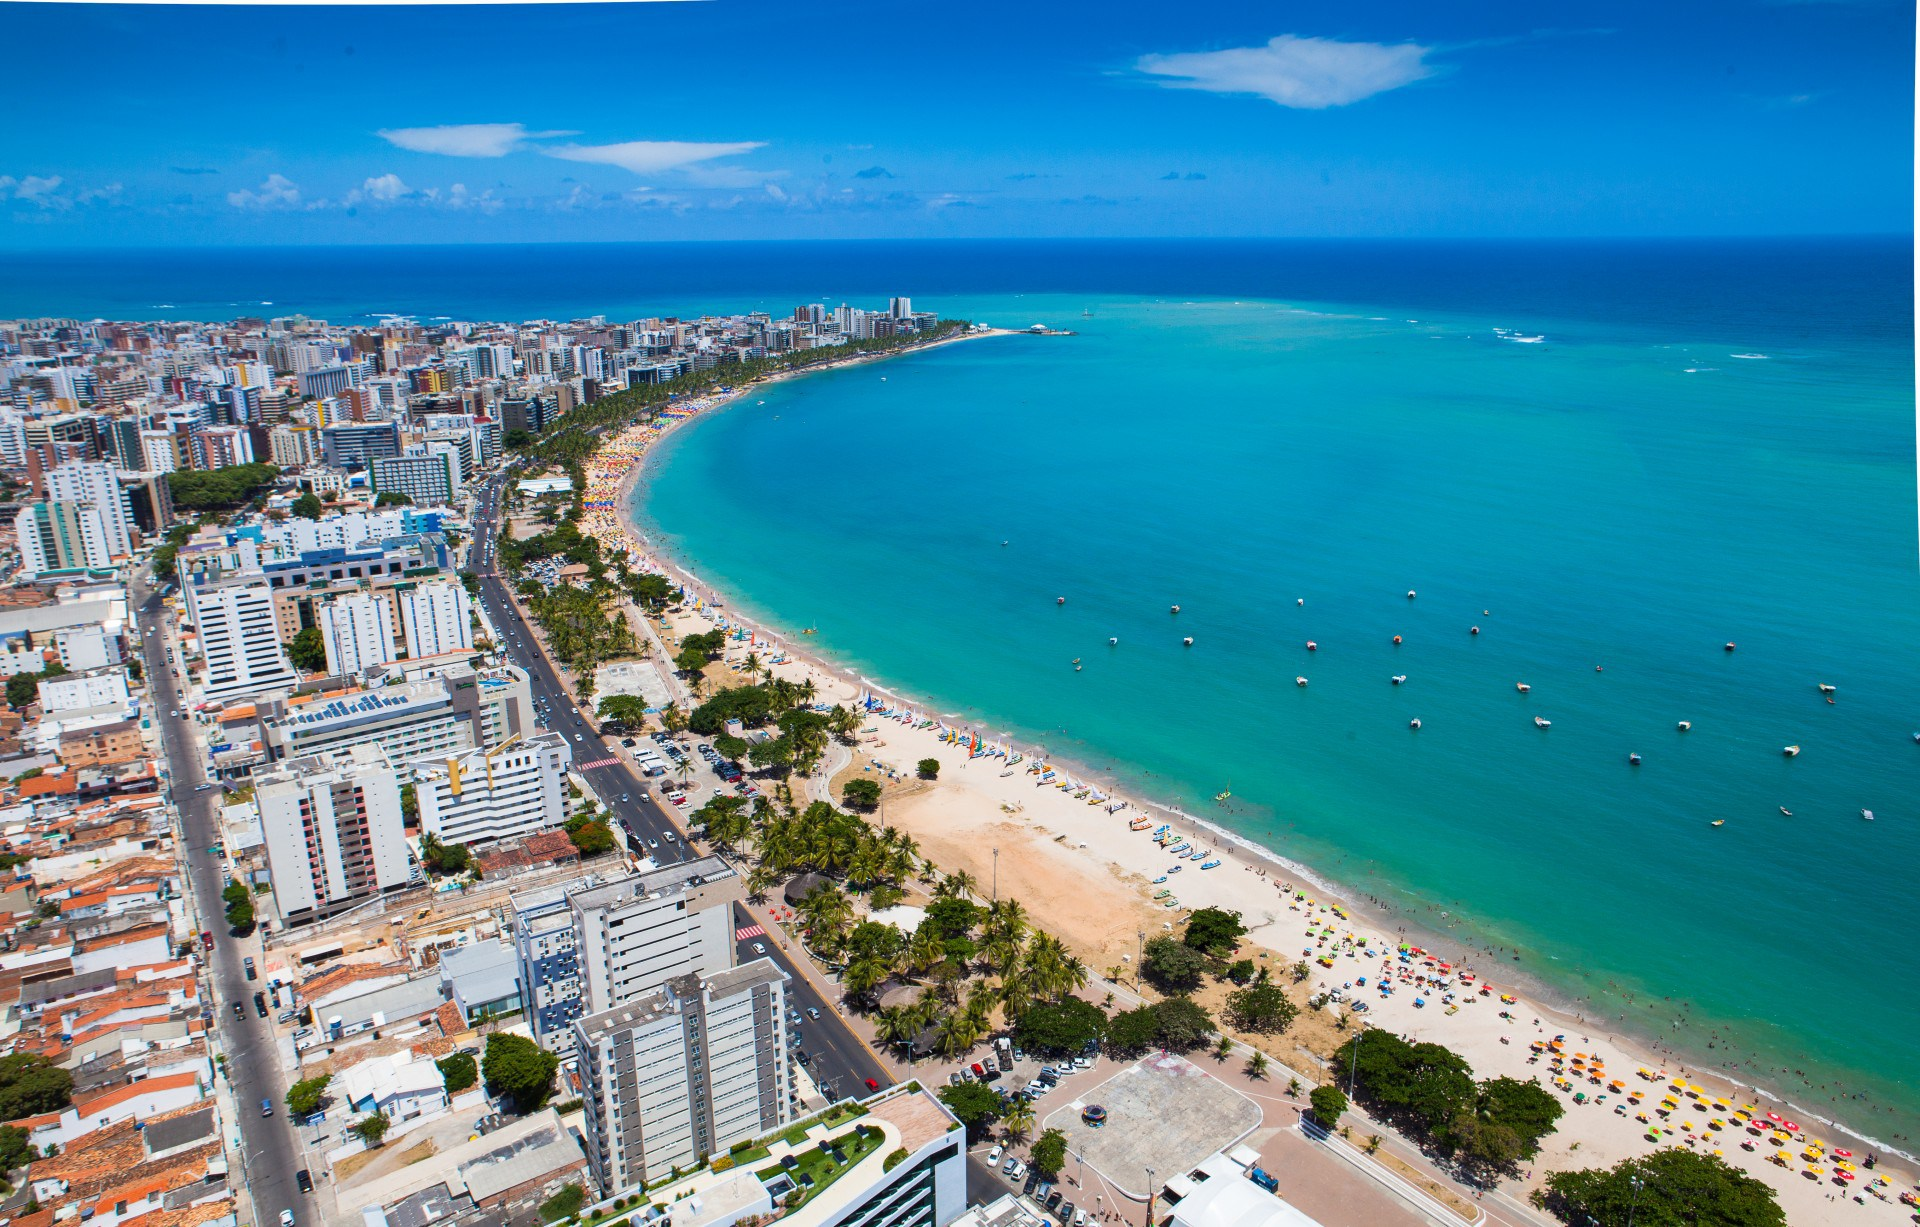
\includegraphics[scale=0.1]{maceio.jpg}
\end{figure}

\begin{figure}[h]
	\centering
	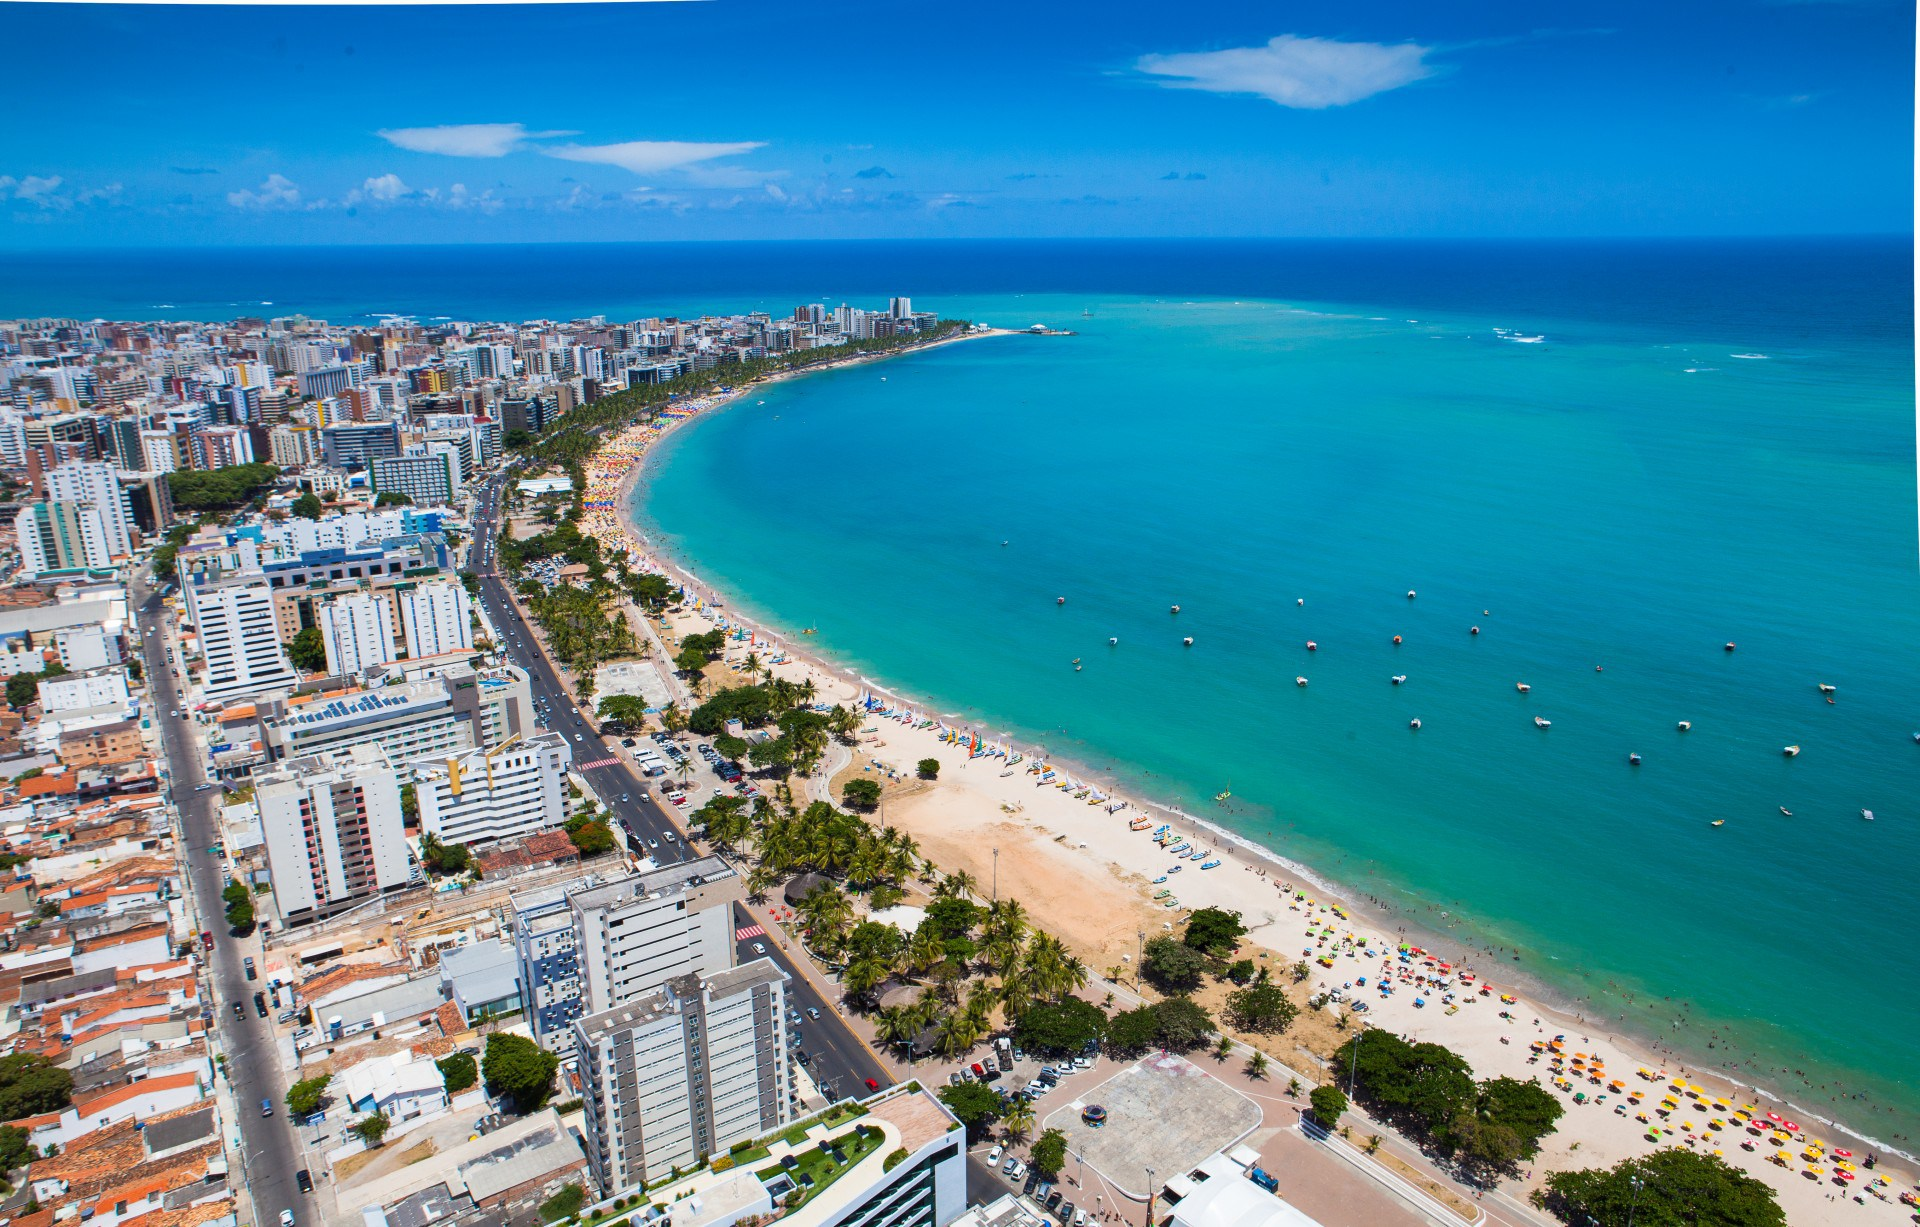
\includegraphics[width=0.5\textwidth]{maceio.jpg}
	\caption{Essa figura ocupa 50\% da largura.}
\end{figure}

\begin{figure}[h]
	\centering
	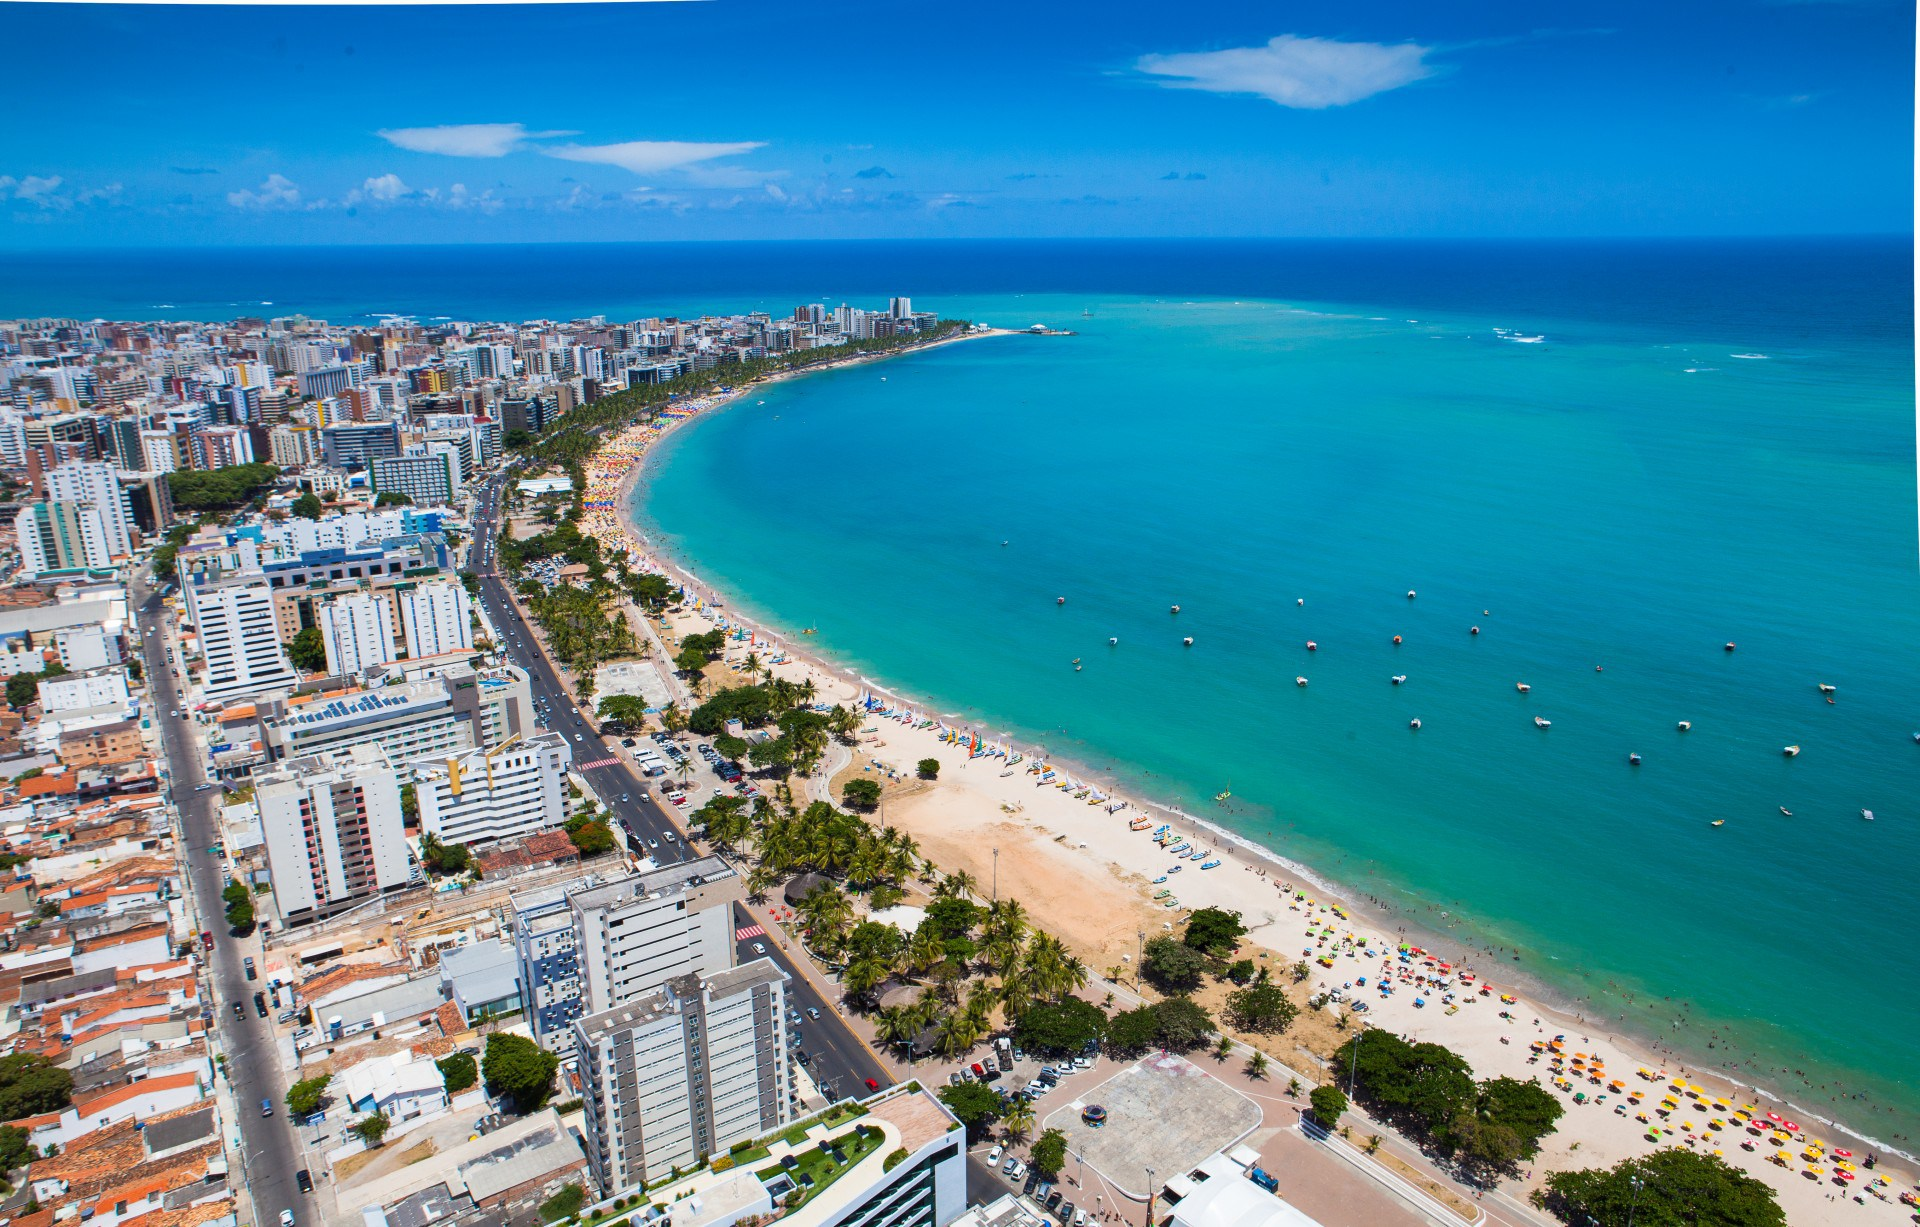
\includegraphics[height=0.3\textheight]{maceio.jpg}
	\caption{Essa figura ocupa 30\% da altura.}
\end{figure}

\begin{figure}[h]
	\centering
	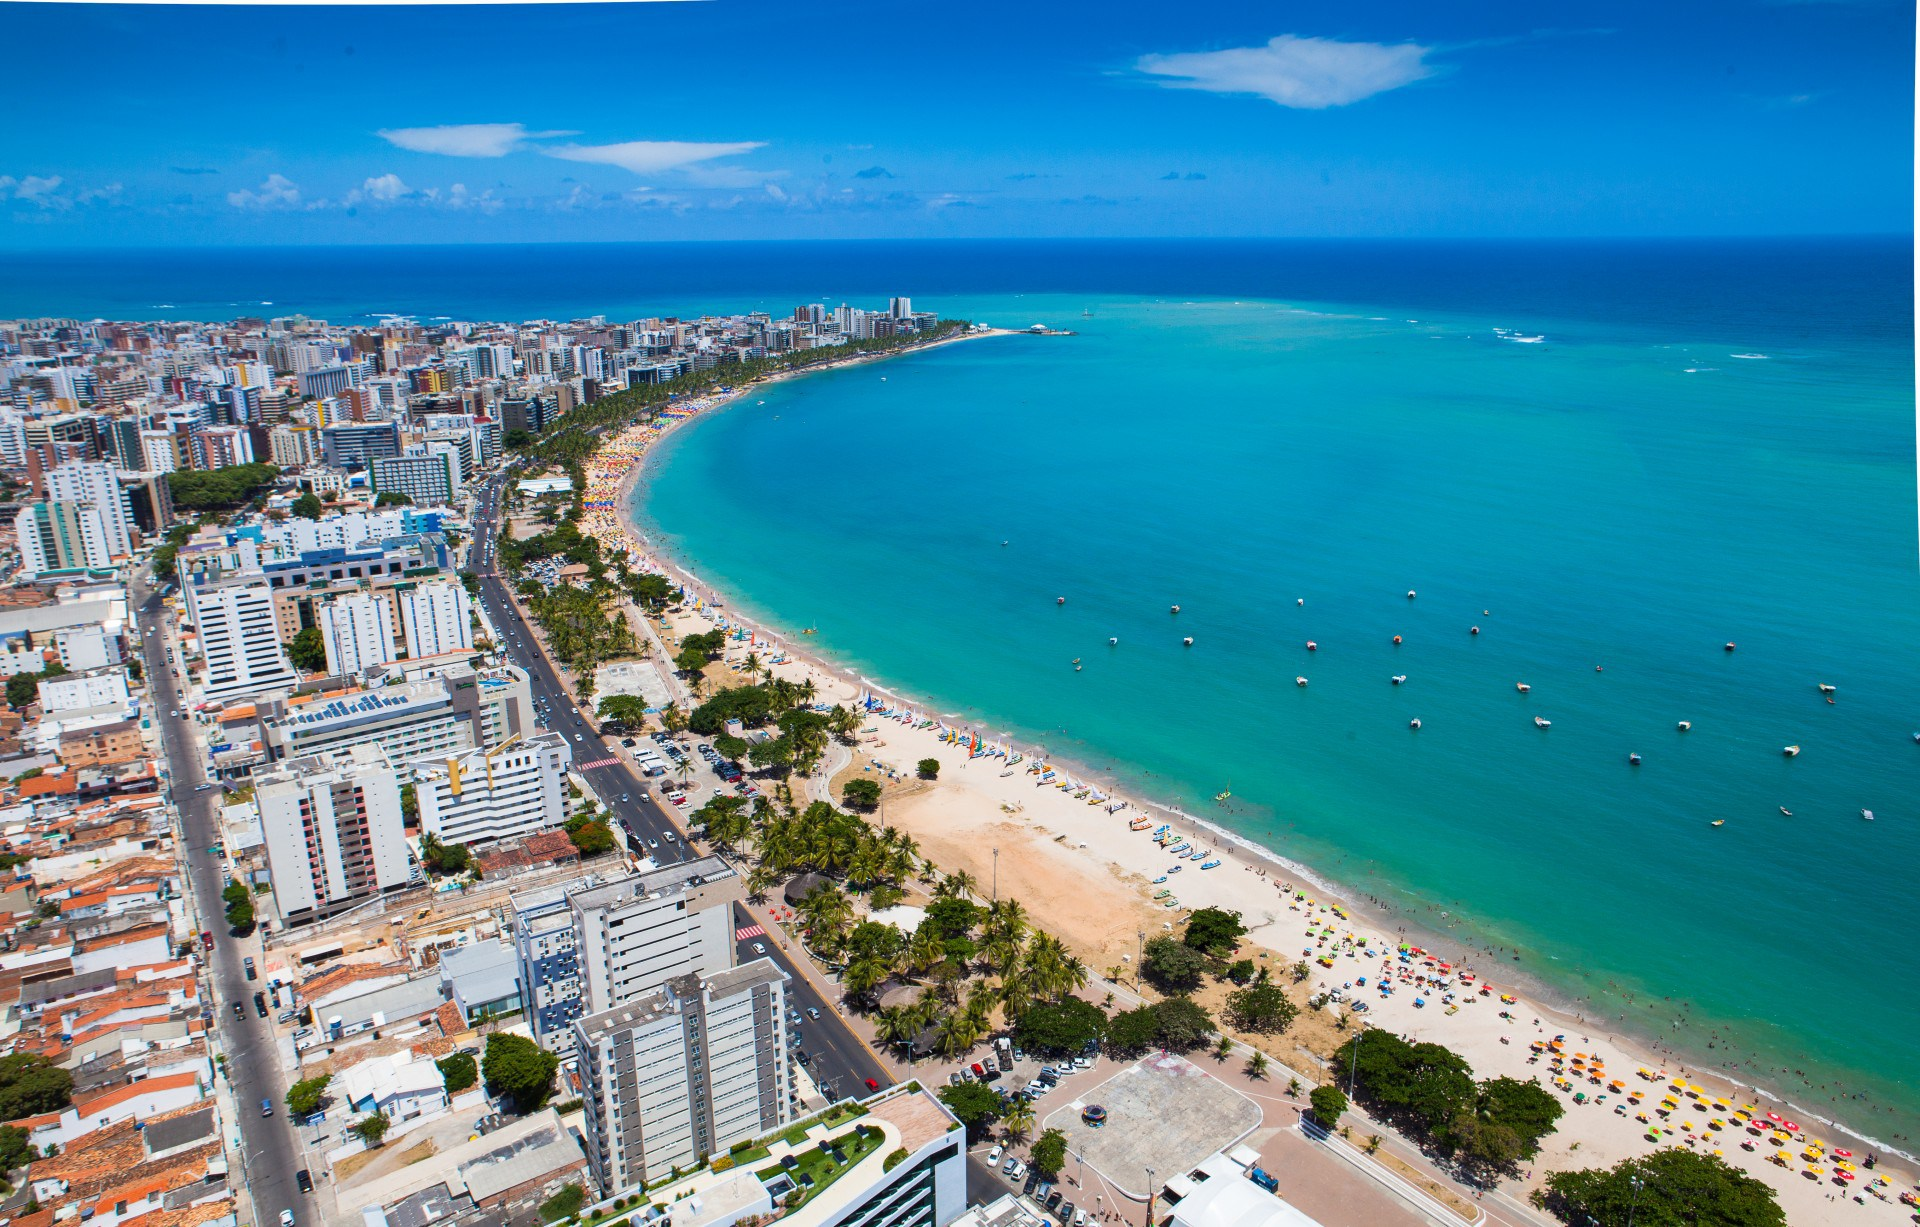
\includegraphics[width=0.4\textwidth]{maceio.jpg}
	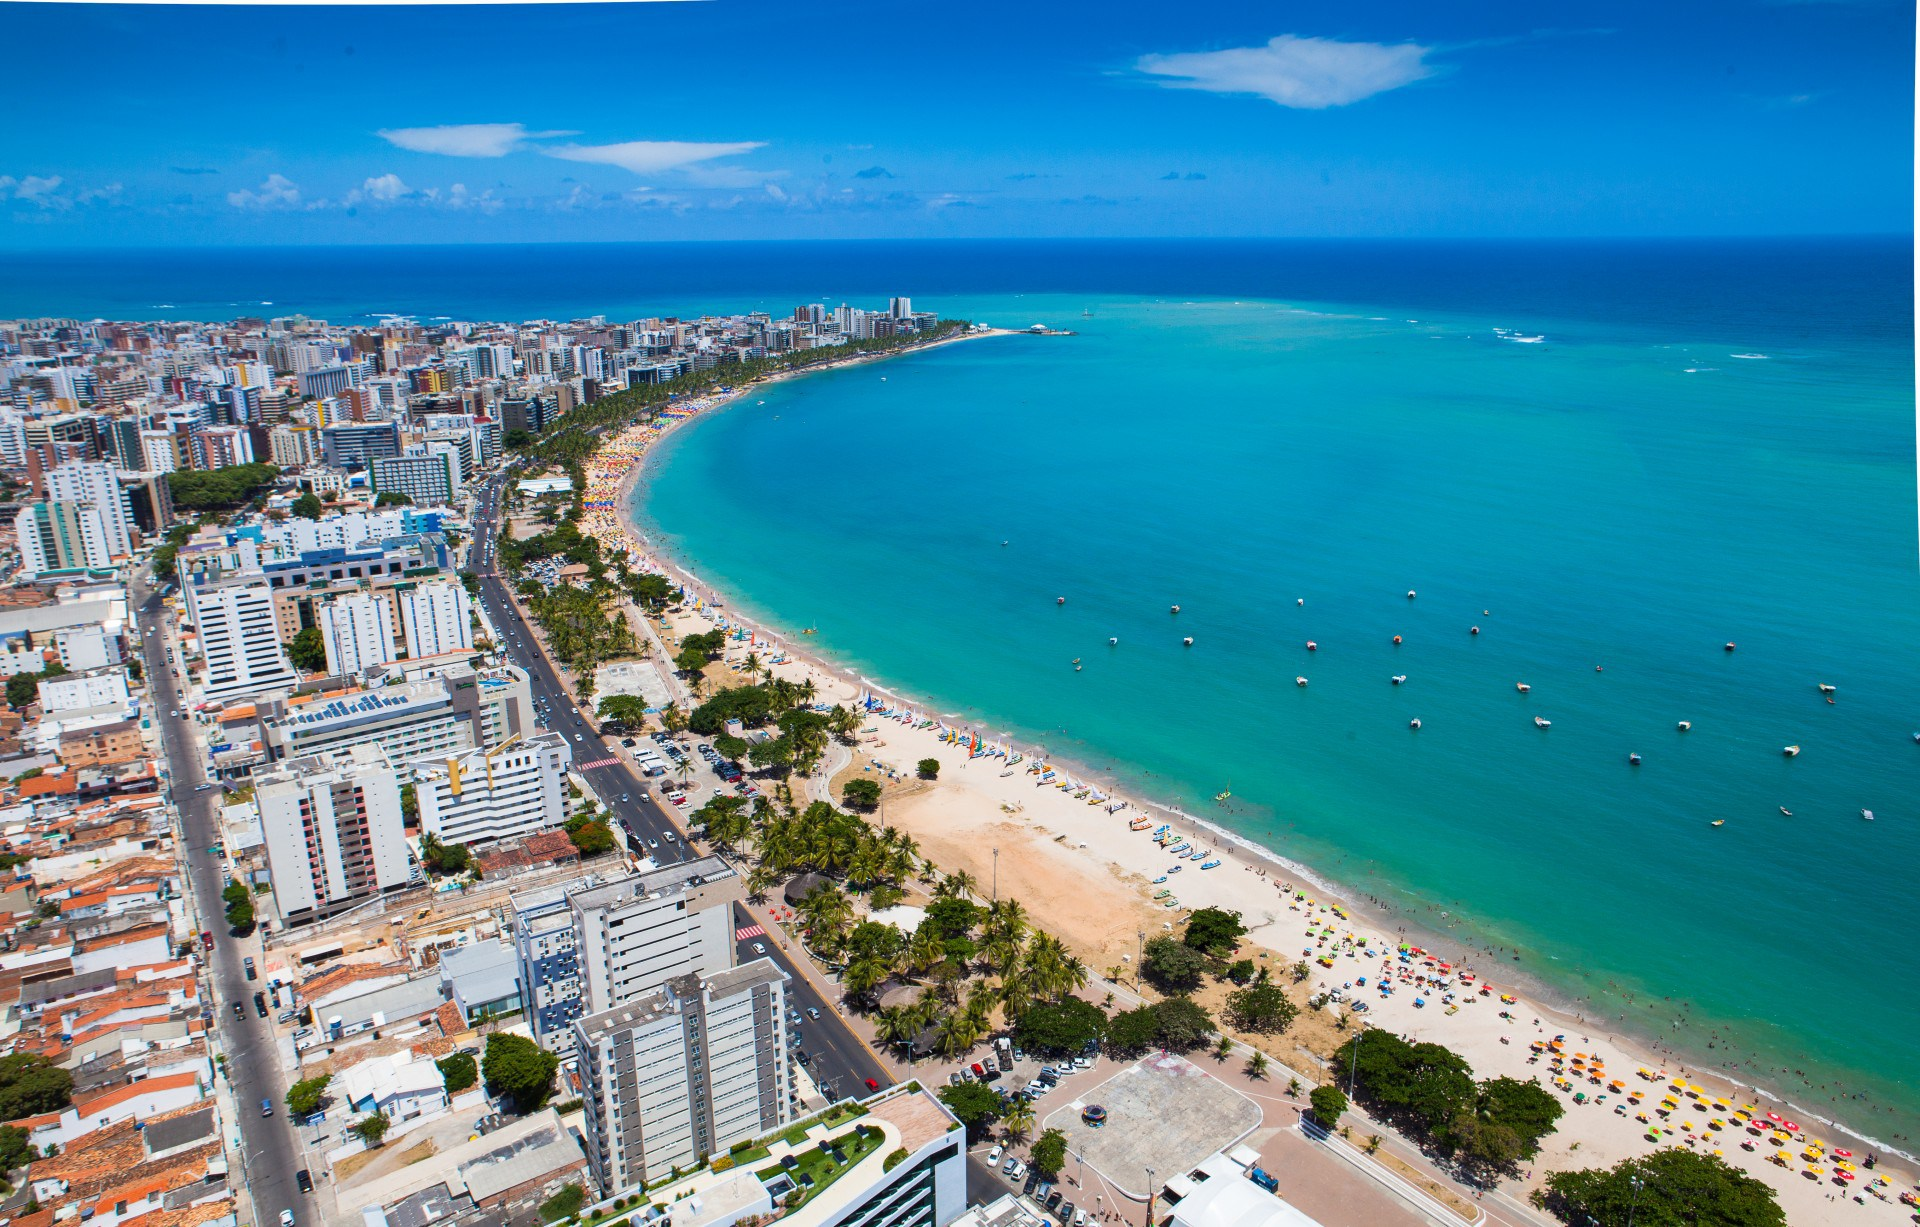
\includegraphics[width=0.4\textwidth]{maceio.jpg}
	\caption{Duas figuras na mesma linha.}
\end{figure}

\begin{figure}
	\begin{subfigure}{0.5\textwidth}
		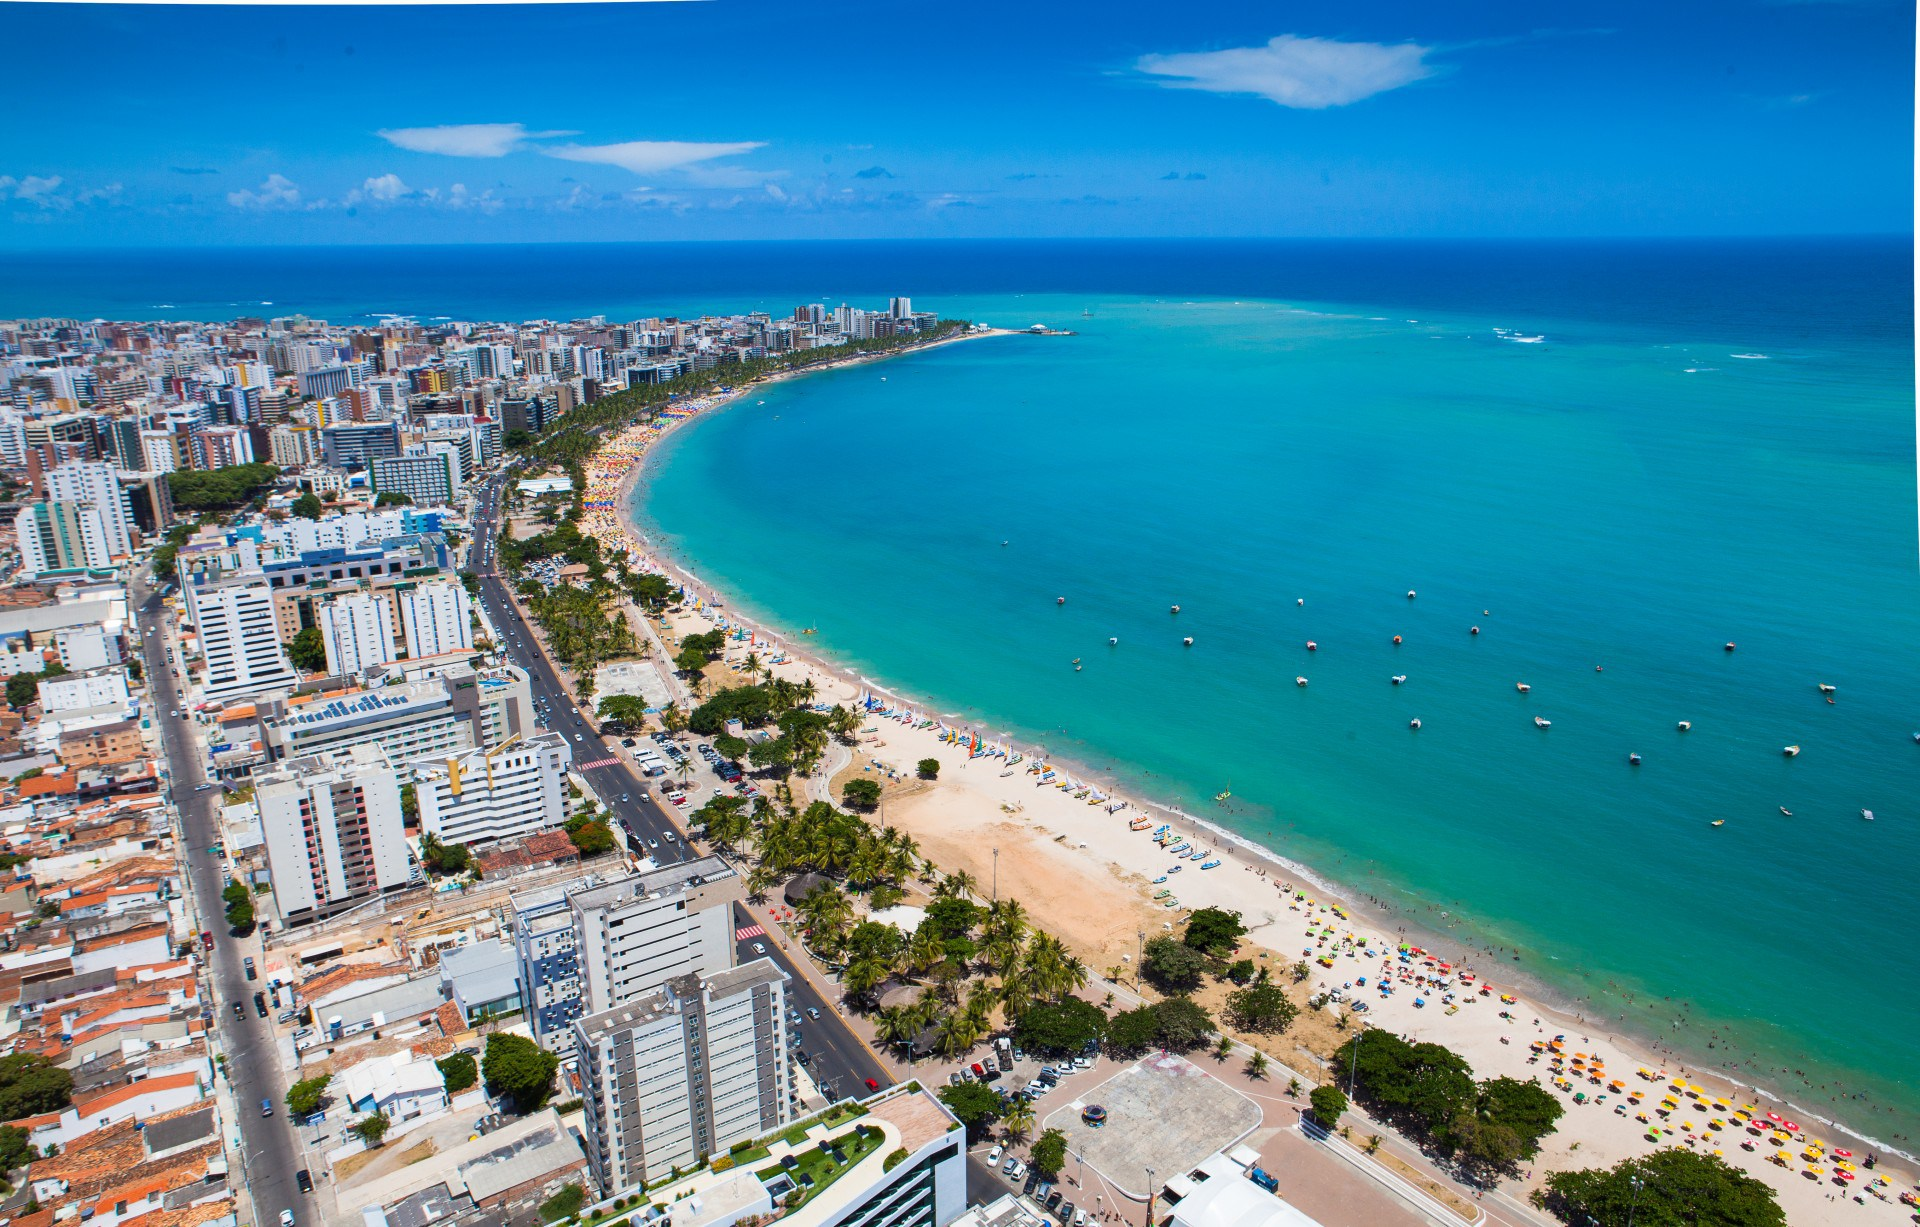
\includegraphics[width=\textwidth]{maceio.jpg}
		\caption{Legenda da primeira figura.}
		\label{subfigure1}
	\end{subfigure}
	\begin{subfigure}{0.5\textwidth}
		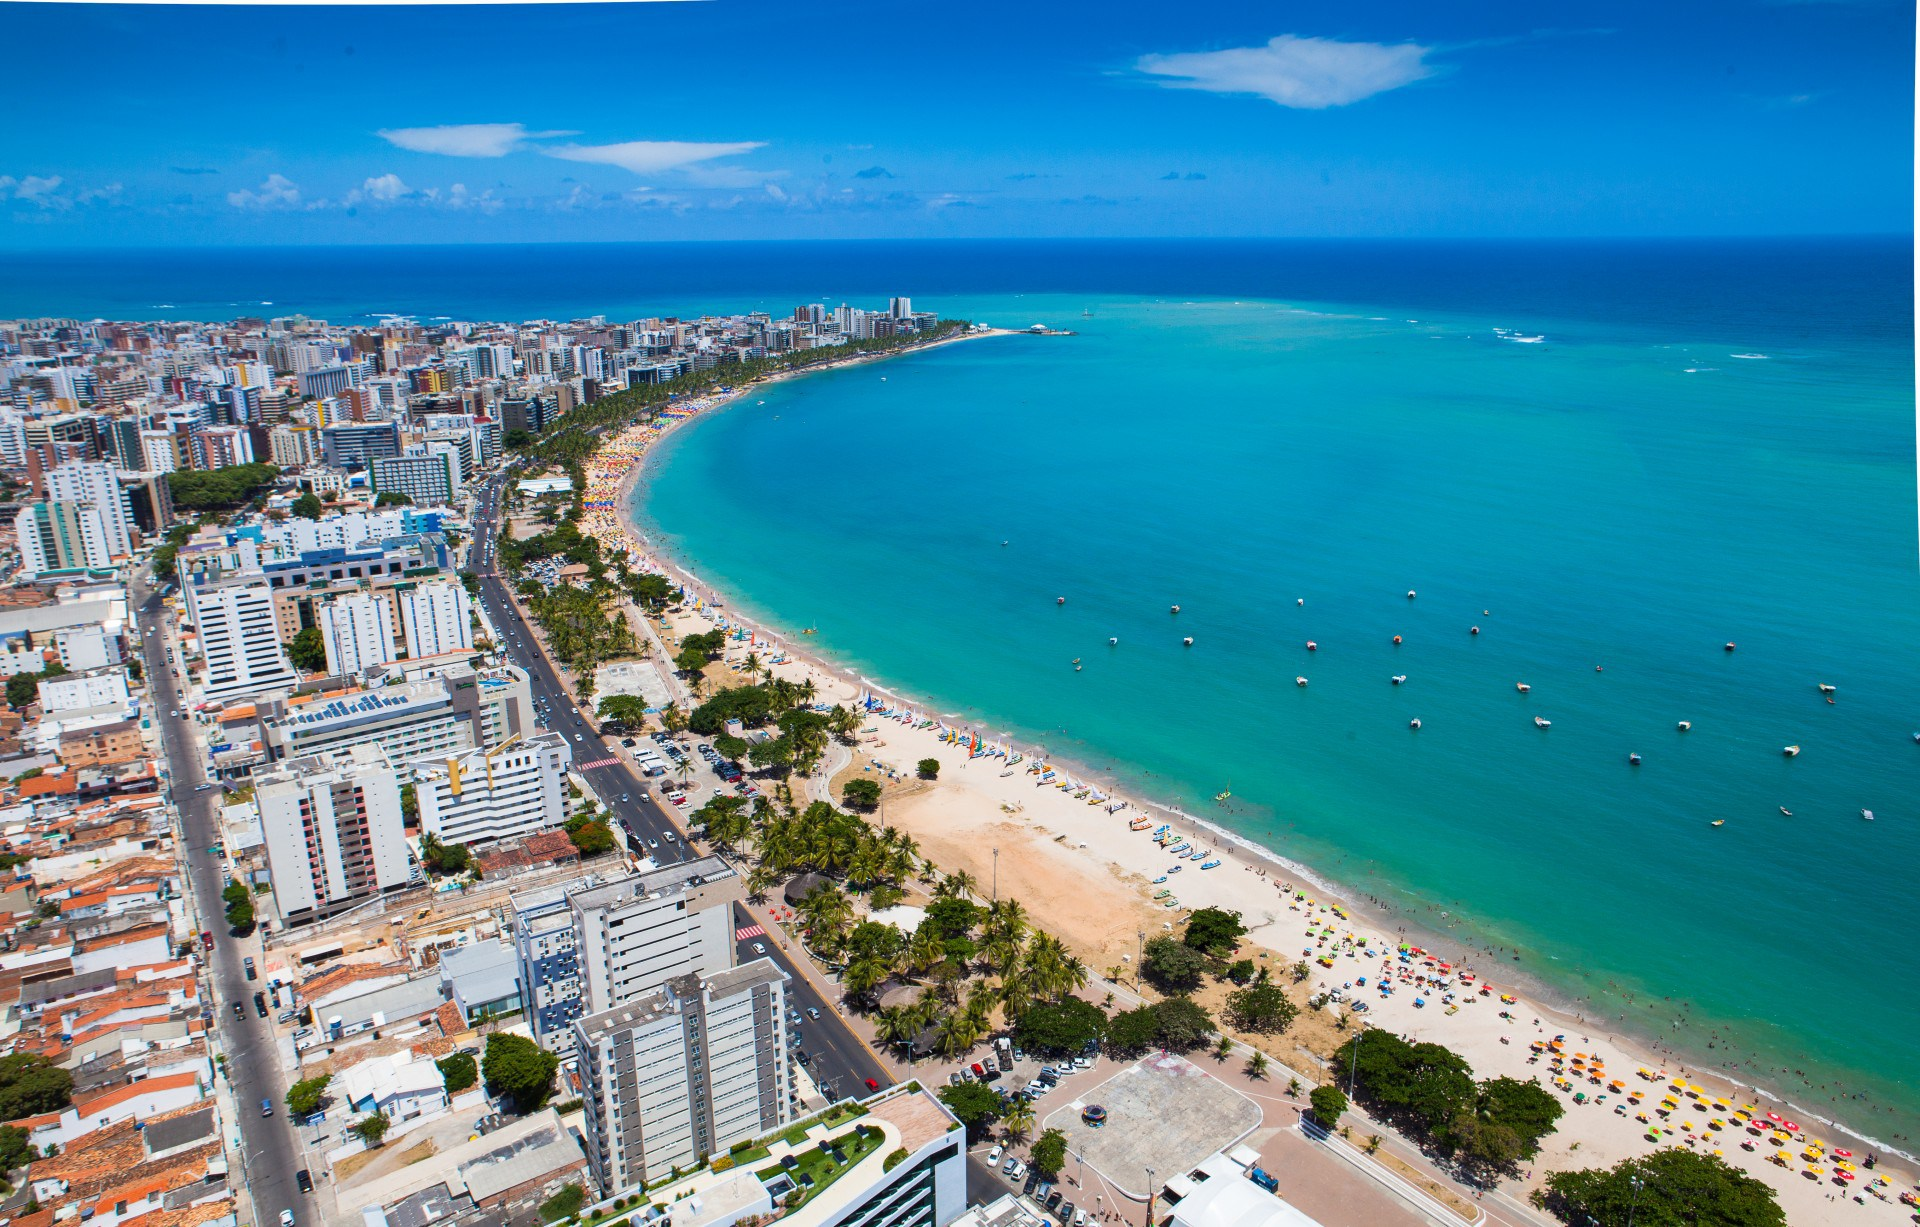
\includegraphics[width=\textwidth]{maceio.jpg}
		\caption{Legenda da segunda figura.}
		\label{subfigure2}
	\end{subfigure}
	\caption{Legenda geral.}
\end{figure}

Referenciando as figuras \ref{subfigure1}, \ref{subfigure2}.

\chapter{Tabelas}
Uma tabela:
\begin{table}[h]
	\centering
	\begin{tabular}{|c|c|}
		\hline
		a & b \\
		\hline
		c & d \\
		\hline
	\end{tabular}
	\caption{Primeira tabela.}
\end{table}

Outra tabela:
\begin{table}[h]
	\centering
	\caption{Essa tabela tem legenda em cima e colunas de 5 cm.}
	\begin{tabular}{|p{5cm}|p{5cm}|}
		\hline
		a & b \\
		\hline
		c & d \\
		\hline
	\end{tabular}
\end{table}

\chapter{Citações}

Citando um autor\cite{calculo}.

Outro autor\cite{kelp}.

% apendices
\begin{apendicesenv}

% Imprime uma página indicando o início dos apêndices
\partapendices

% ----------------------------------------------------------
\chapter{Quisque libero justo}
% ----------------------------------------------------------

\lipsum[50]

% ----------------------------------------------------------
\chapter{Nullam elementum urna vel imperdiet sodales elit ipsum pharetra ligula
ac pretium ante justo a nulla curabitur tristique arcu eu metus}
% ----------------------------------------------------------
\lipsum[55-57]

\end{apendicesenv}

% anexos
\begin{anexosenv}

% Imprime uma página indicando o início dos anexos
\partanexos

% ---
\chapter{Morbi ultrices rutrum lorem.}
% ---
\lipsum[30]

% ---
\chapter{Cras non urna sed feugiat cum sociis natoque penatibus et magnis dis
parturient montes nascetur ridiculus mus}
% ---

\lipsum[31]

% ---
\chapter{Fusce facilisis lacinia dui}
% ---

\lipsum[32]

\end{anexosenv}

% elementos postextuais
\postextual

% bibliografia
%\bibliographystyle{plain}
\bibliography{bibliografia}

% indice remissivo
\phantompart
\printindex

\end{document}
